\documentclass{standalone}
\usepackage{tikz}
\begin{document}
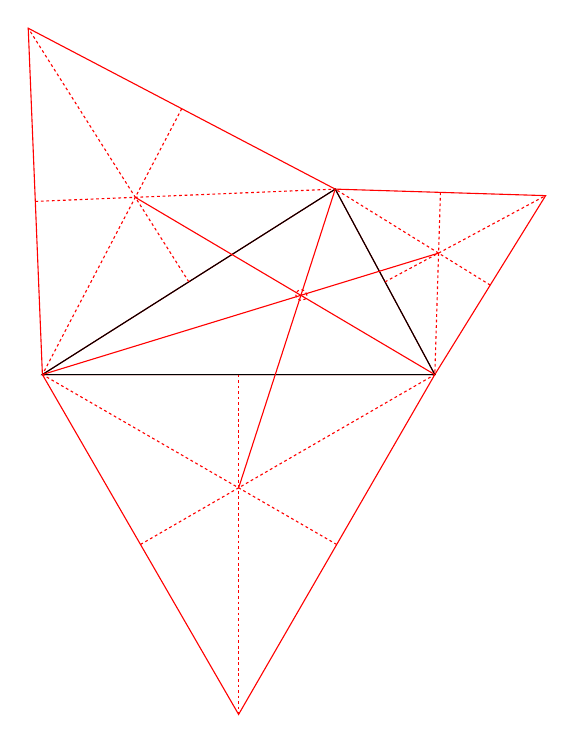
\begin{tikzpicture}[x=1pt,y=1pt]
\draw[red] (207.68,-84.26) -- (131.66,-81.91) -- (167.64,-148.92) -- cycle;
\draw[red] (20.72,-23.77) -- (25.84,-148.92) -- (131.66,-81.91) -- cycle;
\draw[red] (25.84,-148.92) -- (96.74,-271.72) -- (167.64,-148.92) -- cycle;
\draw (25.84,-148.92) -- (167.64,-148.92) -- (131.66,-81.91) -- cycle;
\draw[red] (59.40,-84.87) -- (167.63,-148.92);
\draw[red] (25.84,-148.92) -- (169.00,-105.02);
\draw[red] (131.66,-81.91) -- (96.75,-189.86);
\draw[red, dash pattern=on 1pt] (78.75,-115.41) -- (20.72,-23.77);
\draw[red, dash pattern=on 1pt] (76.19,-52.84) -- (25.84,-148.92);
\draw[red, dash pattern=on 1pt] (23.29,-86.35) -- (131.66,-81.91);
\draw[red, dash pattern=on 1pt] (96.74,-148.92) -- (96.74,-271.72);
\draw[red, dash pattern=on 1pt] (132.19,-210.31) -- (25.85,-148.92);
\draw[red, dash pattern=on 1pt] (61.29,-210.31) -- (167.63,-148.92);
\draw[red, dash pattern=on 1pt] (169.68,-83.08) -- (167.64,-148.92);
\draw[red, dash pattern=on 1pt] (149.65,-115.41) -- (207.68,-84.25);
\draw[red, dash pattern=on 1pt] (187.67,-116.59) -- (131.66,-81.91);
\draw[red, dash pattern=on 1pt] (119.42,-120.18) circle (2.00);
\end{tikzpicture}
\end{document}
